\documentclass{article}
\begin{document}
\subsection{Running examples on PC side}
\subsubsection{Working principle}
When compiling the COINES SDK for PC side, the COINES layer provides an abstraction of the embedded environment on the host side. COINES library provides read and write functions for I\textsuperscript{2}C and SPI on PC side. These functions receive the arguments of the user input (i.e. what register address to read from) and tunnel them through the USB connection to the Application Board, where they are fed into the embedded I\textsuperscript{2}C and SPI functions and are executed to access the sensor. Any result or response from those functions is tunneled back to the PC side and provided to the example application.

This approach allows easy and flexible programming and offers the possibility to integrate the example code into other applications or add advanced logging options. The drawback is that in this mode the code is not executed in real time, as it runs on a multi-tasking operating system. To overcome this drawback, the examples can also be run on the MCU side (see section \ref{ExampleOnMCU}).

\begin{figure}[H]
	\begin{center}
		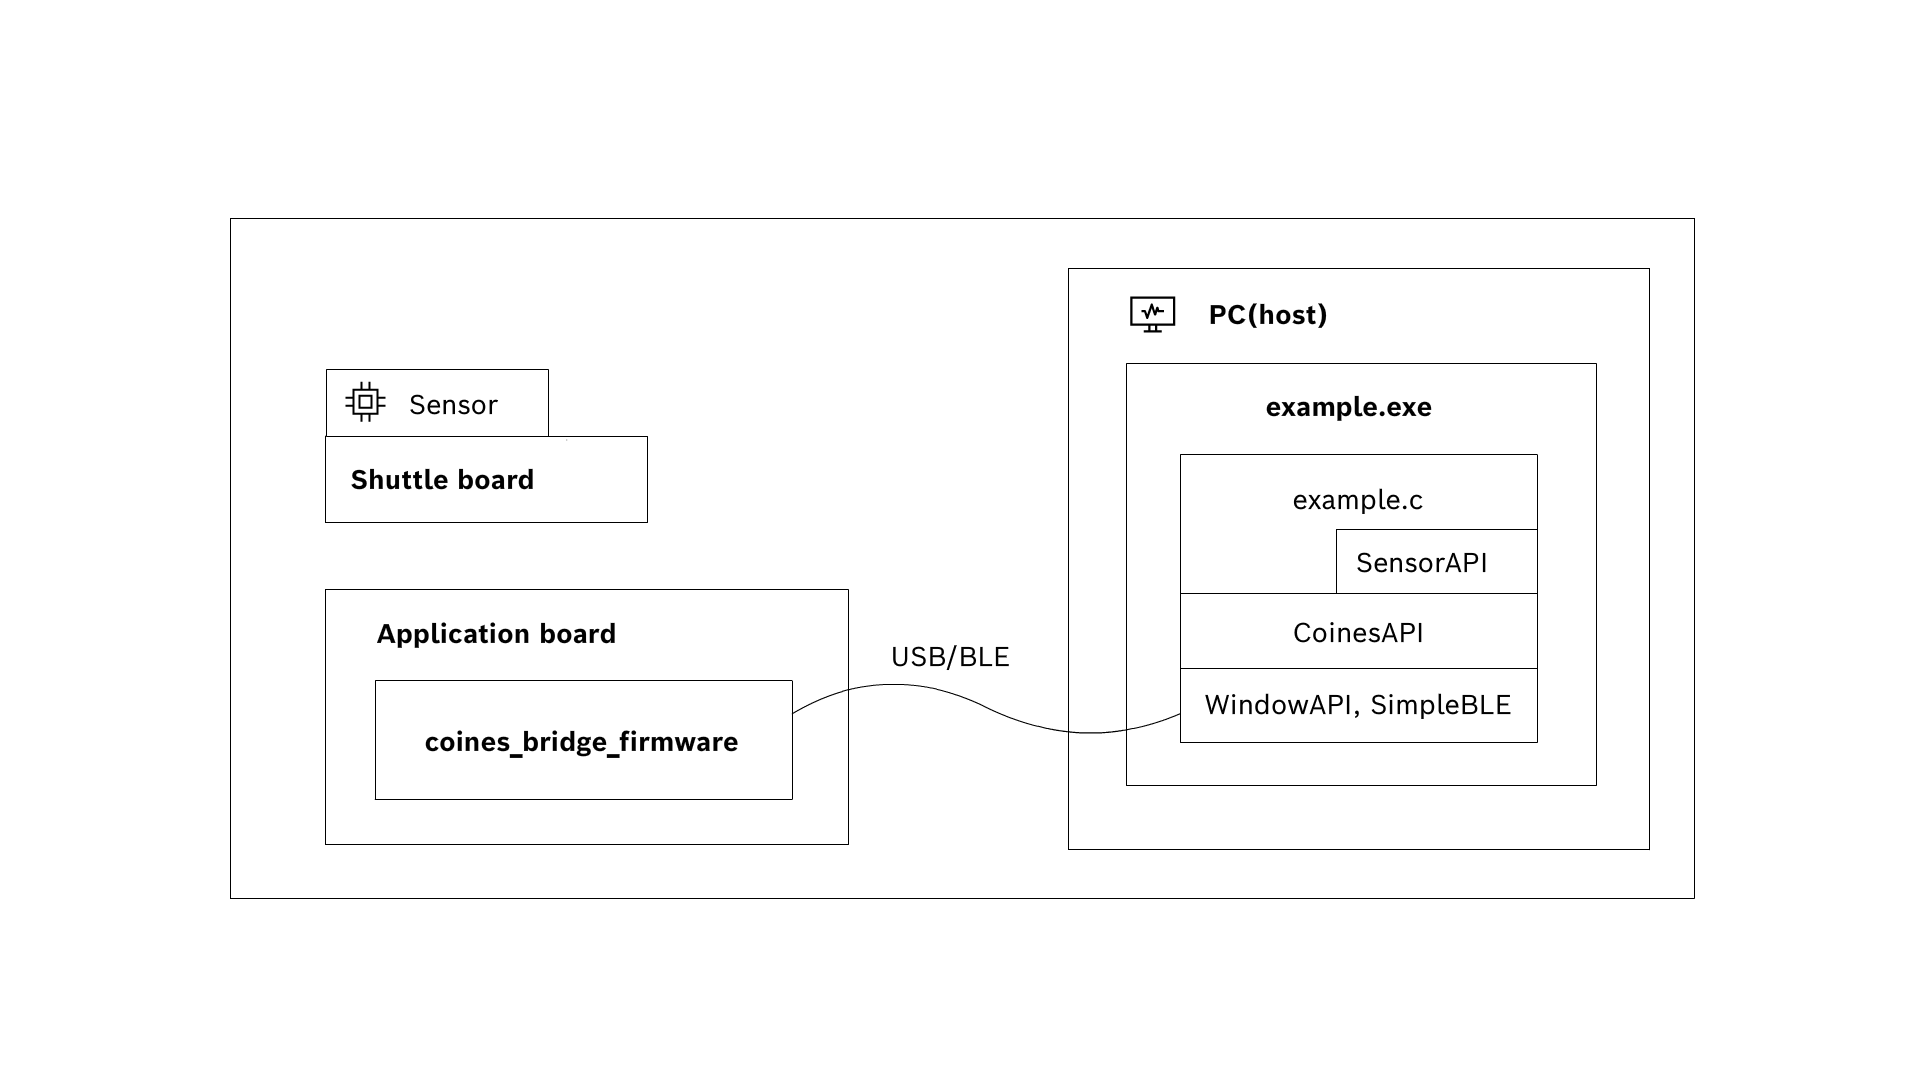
\includegraphics[width=0.9\textwidth]{coinesAPI_images/COINES_workingPrinciple_runOnPC.png}
		\caption{Working principle: Running example on PC side}
	\end{center}
\end{figure}

\subsubsection{PC side implementation}
This setup has the challenge of lacking the real-time capabilities known from a pure microcontroller environment. To overcome this, the coinesAPI offers streaming functions, which allow the user to schedule data readout directly on the microcontroller, either based on a data interrupt coming from the sensors or based on the timer of the microcontroller. The scheduler waits for the configured interrupt (sensor interrupt or timer interrupt) and reads out areas of the register map, which can be configured by the user.

As an example, the user could choose to read out the 6 bytes from the register map of a certain inertial sensor, containing the sensor data of three axis (2 bytes per axis). If the user would configure e.g a readout once per milliseconds, the result would be a data stream of three-axis sensor data at a rate of 1 kHz.

\subsubsection{Getting started}
To get started with example execution, follow these steps:
\begin{enumerate}
\item Connect the Application board via USB, with the sensor shuttle board mounted.
\item Refer to section \ref{firmwareUpdate} and update the Coines Bridge firmware to the board.
\item Open the command prompt or the terminal.
\item Use the command \texttt{cd} to go to the directory where the example that is to be built is located.
\end{enumerate}
Note: Some examples may not compile for both PC and MCU target. Please refer to the example documentation or simply the example name (e.g. examples that can only be compiled for the PC are named with a following '\_pc').

\subsubsection{Interfacing via BLE}
The procedure to interface via BLE involves these steps:
\begin{enumerate}
	\item Open the script to be executed (in case of SensorAPI - common.c file in the selected example folder) in your IDE
	\item Change COINES\_COMM\_INTF\_USB  to COINES\_COMM\_INTF\_BLE
	\item Now follow the steps from 1 - 4 in the above section
\end{enumerate}

\subsubsection{Compiling}
To run an example in PC side, execute below command "mingw32-make TARGET=PC". Use '\texttt{mingw32-make}' (TDM-GCC/MinGW) or '\texttt{make}' (Linux/Cygwin/MSYS2/MacOS) for compilation.

\subsubsection{Viewing the results}
Running the output executable in the command prompt of the PC will display the results. To view ouput via BLE, connect the Application board to another power source and keep it within the BLE range and run the executable in the PC.

\subsubsection{Data logging}

The user can utilize the terminal's output redirection command to store the result of a command/executable in a file, as demonstrated below.
\begin{figure}[H]
	\begin{center}
		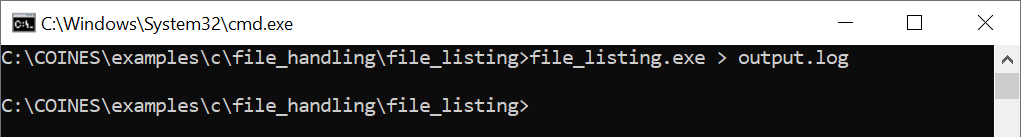
\includegraphics[width=0.9\textwidth]{coinesAPI_images/PC_data_logging.png}
	\end{center}
\end{figure}


\end{document}